\documentclass[11pt,]{article}
\usepackage[left=1in,top=1in,right=1in,bottom=1in]{geometry}
\newcommand*{\authorfont}{\fontfamily{phv}\selectfont}
\usepackage[]{libertine}


  \usepackage[T1]{fontenc}
  \usepackage[utf8]{inputenc}




\usepackage{abstract}
\renewcommand{\abstractname}{}    % clear the title
\renewcommand{\absnamepos}{empty} % originally center

\renewenvironment{abstract}
 {{%
    \setlength{\leftmargin}{0mm}
    \setlength{\rightmargin}{\leftmargin}%
  }%
  \relax}
 {\endlist}

\makeatletter
\def\@maketitle{%
  \newpage
%  \null
%  \vskip 2em%
%  \begin{center}%
  \let \footnote \thanks
    {\fontsize{18}{20}\selectfont\raggedright  \setlength{\parindent}{0pt} \@title \par}%
}
%\fi
\makeatother




\setcounter{secnumdepth}{0}




\title{Modern Statistical Machine Learning Methods Applied to
Airbnb \thanks{Replication files are available on the author's Github
account (\url{https://github.com/wangqinz}). \textbf{Current version}:
January 22, 2022; \textbf{Corresponding author}:
\href{mailto:qinzhe.wang@duke.edu}{\nolinkurl{qinzhe.wang@duke.edu}}.}  }
 



\author{\Large Qinzhe Wang\vspace{0.05in} \newline\normalsize\emph{Duke
University}  }


\date{}

\usepackage{titlesec}

\titleformat*{\section}{\normalsize\bfseries}
\titleformat*{\subsection}{\normalsize\itshape}
\titleformat*{\subsubsection}{\normalsize\itshape}
\titleformat*{\paragraph}{\normalsize\itshape}
\titleformat*{\subparagraph}{\normalsize\itshape}


\usepackage{natbib}
\bibliographystyle{apsr}
\usepackage[strings]{underscore} % protect underscores in most circumstances



\newtheorem{hypothesis}{Hypothesis}
\usepackage{setspace}


% set default figure placement to htbp
\makeatletter
\def\fps@figure{htbp}
\makeatother

\usepackage{hyperref}
\usepackage{array}
\usepackage{caption}
\usepackage{graphicx}
\usepackage{siunitx}
\usepackage[table]{xcolor}
\usepackage{multirow}
\usepackage{hhline}
\usepackage{calc}
\usepackage{tabularx}
\usepackage{fontawesome}
\usepackage[para,online,flushleft]{threeparttable}
\usepackage{booktabs}
\usepackage{longtable}
\usepackage{array}
\usepackage{multirow}
\usepackage{wrapfig}
\usepackage{float}
\usepackage{colortbl}
\usepackage{pdflscape}
\usepackage{tabu}
\usepackage{threeparttable}
\usepackage{threeparttablex}
\usepackage[normalem]{ulem}
\usepackage{makecell}
\usepackage{xcolor}

% move the hyperref stuff down here, after header-includes, to allow for - \usepackage{hyperref}

\makeatletter
\@ifpackageloaded{hyperref}{}{%
\ifxetex
  \PassOptionsToPackage{hyphens}{url}\usepackage[setpagesize=false, % page size defined by xetex
              unicode=false, % unicode breaks when used with xetex
              xetex]{hyperref}
\else
  \PassOptionsToPackage{hyphens}{url}\usepackage[draft,unicode=true]{hyperref}
\fi
}

\@ifpackageloaded{color}{
    \PassOptionsToPackage{usenames,dvipsnames}{color}
}{%
    \usepackage[usenames,dvipsnames]{color}
}
\makeatother
\hypersetup{breaklinks=true,
            bookmarks=true,
            pdfauthor={Qinzhe Wang (Duke University)},
             pdfkeywords = {Random Forest, AdaBoost, Logistic
Regression},  
            pdftitle={Modern Statistical Machine Learning Methods
Applied to Airbnb},
            colorlinks=true,
            citecolor=blue,
            urlcolor=blue,
            linkcolor=magenta,
            pdfborder={0 0 0}}
\urlstyle{same}  % don't use monospace font for urls

% Add an option for endnotes. -----


% add tightlist ----------
\providecommand{\tightlist}{%
\setlength{\itemsep}{0pt}\setlength{\parskip}{0pt}}

% add some other packages ----------

% \usepackage{multicol}
% This should regulate where figures float
% See: https://tex.stackexchange.com/questions/2275/keeping-tables-figures-close-to-where-they-are-mentioned
\usepackage[section]{placeins}


\begin{document}
	
% \pagenumbering{arabic}% resets `page` counter to 1 
%    

% \maketitle

{% \usefont{T1}{pnc}{m}{n}
\setlength{\parindent}{0pt}
\thispagestyle{plain}
{\fontsize{18}{20}\selectfont\raggedright 
\maketitle  % title \par  

}

{
   \vskip 13.5pt\relax \normalsize\fontsize{11}{12} 
\textbf{\authorfont Qinzhe Wang} \hskip 15pt \emph{\small Duke
University}   

}

}








\begin{abstract}

    \hbox{\vrule height .2pt width 39.14pc}

    \vskip 8.5pt % \small 

\noindent Airbnb is one of the most popular room-booking platforms. The
majority of bookings go successfully. However, some may run into a
problem with availability. My research attempts to help consumers avoid
being unable to book their favorite listings by examining how numerous
criteria such as location, host, property condition, and seasonality,
affect listing availability. More specifically, I consider regional data
from Asheville, North Carolina, which is considered a tourist
destination and is increasing in its popularity with regard to bookings.
Motivated as such, I consider a data set from Inside Airbnb Data
Platform, which covers such data as already mentioned. This data set has
both categorical and numerical predictors. The primary choices of models
are AdaBoost, regarding decision trees as weak leaners, and Random
Forest. On the one hand, both models perform well in a dataset
containing both categorical and numerical predictors. On the other hand,
ensemble learning methods usually outperform a single tree (CART) with
bagging (Random Forest) and boosting (AdaBoost) techniques to reduce the
dispersion of the predictions. I trained each technique, tuned
hyper-parameters, and evaluated performance with K-fold
cross-validation, using accuracy rate as the evaluation metric. In
addition, I connected the top 5 most important features to real-world
reasons.


\vskip 8.5pt \noindent \emph{Keywords}: Random Forest, AdaBoost,
Logistic Regression \par

    \hbox{\vrule height .2pt width 39.14pc}



\end{abstract}


\vskip -8.5pt


 % removetitleabstract

\noindent  

\hypertarget{introduction-and-dataset}{%
\section{1 Introduction and dataset}\label{introduction-and-dataset}}

The project's primary focus is forecasting whether or not an Airbnb
listing is available, which is a classification problem. The dataset is
from Inside Airbnb Data Platform with 7471 observations and 22
variables, including hosting characteristics, room information, room
type, and reviews. In addition, the dataset contains 2139 missing
values. The dependent variable Decision is binary, with 1 standing for
available and 0 for unavailable. The dataset is quite balanced.

\hypertarget{data-cleaning}{%
\section{2 Data Cleaning}\label{data-cleaning}}

There are four groups of features in the dataset, excluding avaliability
(the dependent varaible)

\textbf{Host Characteristics}: Four features are associated with host
information, including Host\_response\_time, Host\_is\_superhost,
Host\_has\_profile\_pic, and Host\_identity\_verified. All four features
are binary, with 1 for ``Yes'' and 0 for ``No''. For all features,
missing values are recoded as a different group, named unknown.

\textbf{Room Information}: Room Information includes Price,
Neighbourhood, Bathroom\_text, Bedrooms, Beds, Balcony, Parking, and
Cooking. Regular expressions are applied to price to remove the dollar
sign in the front and the commas between numbers. In addition, the
distribution of price is right-skewed; therefore, a log transformation
is applied. Variable Bathroom\_text is formatted as strings, containing
two parts of information: the number of bathrooms and the bathroom type.
Splitting the string into two the above parts is necessary. Bedrooms and
Beds contain a number of missing values, but they can be imputed. The
distributions of both features are right-skewed with the Pearson
correlation coefficient of 0.85 approximately. Therefore I used the
median value of Bedrooms to impute the missing value in Beds and vice
versa. There are still some missing values remaining. One potential
solution is to use the median number of bathrooms to fill because the
Pearson correlation coefficient between the number of bedrooms and the
number of bathrooms is 0.81 approximately.

\textbf{Room Type}: There are 55 different property types, and the
availability ratios and the sample sizes are different across all 55
groups. Some groups have extremely small sample sizes; thus, aggregating
them can be a choice. Regarding 100 as the cutoff points of group sample
size, property type groups with sizes greater than 100 remain the same.
For other property types, if the type name contains text ``private'' or
``entire'', they can be treated as ``Private small room''; if the
Property\_type contains the text ``shared'', they can be treated as
``Share small room''. Otherwise, they are aggregated to group ``Other''.

\textbf{Reviews}: A dummy variable is created instead of
Number\_of\_reviews because the overall pricing is significantly
different between listings having reviews and listing without reviews.

\hypertarget{methods}{%
\section{Methods}\label{methods}}

\hypertarget{cross-validation-and-evaluation-metrics}{%
\subsection{Cross-validation and Evaluation
Metrics}\label{cross-validation-and-evaluation-metrics}}

Before introducing methods, the dataset is split into two parts,
self-contributed training and testing. The proportion of testing data is
0.3. 5-fold cross-validation is applied to avoid overfitting. Models are
trained and tuned hyperparameters in the self-contributed training
dataset and predicted in the self-contributed testing dataset. The
accuracy ratio is the choice of evaluation metric because it simply
measures how often the classifier correctly predicts. Since our goal is
to predict the availability of Airbnb listings based on balanced data,
the accuracy ratio is useful when the target class is well balanced.

\hypertarget{logistic-regression}{%
\subsection{Logistic Regression}\label{logistic-regression}}

Logistic regression is easy to train and interpret, providing a general
view of the pre-processing quality. In addition, there are not many
parameters that need to be tuned in logistic regression, except the
penalization. Penalized logistic regression imposes a penalty for having
too many variables. With L2 penalty and 5-fold cross-validation inside
the self-contributed training dataset to tune the penalty strength. Most
often the penalty term is \(\lambda \sum \theta_j ^2\), and
\(C = \frac{1}{\lambda}\). The choice of penalty strength C can be
selected from \(10^{-6}, 10^{-5},\cdots, 10^6\). Although a larger value
of C lowers the strength of regularization, the purpose of the selection
is to visualize the training \& testing accuracy and the time. The
result of the grid search suggests C = 100 (\(\lambda = 0.01\)) as the
optimal hyperparameter. The overall accuracy is 0.70 on the training
dataset and 0.69 on the testing dataset.

\hypertarget{random-forest}{%
\subsection{Random Forest}\label{random-forest}}

The second method is the random forest, which uses bagging to select the
subset of observation \& features and uses majority vote to classify.
Instead of searching for the most critical feature while splitting a
node as a decision tree does, it adds additional randomness to the
model, finds the best features among randomly selected subsets of
features, resulting in a wide diversity. In addition, Random Forest
performs well to solve non-linearity problems. And it can handle
high-dimension datasets. The last important reason is that Random Forest
can handle missing values and outliers. Even though there is no missing
value after the pre-processing process, Random Forest is a good try. One
noteworthy point is that we will get different results if we perform
random forest in both R and Python. The function in sklearn.ensemble
package (Python) averages the probabilistic predictions of each tree
while the function in R uses the majority votes. I did in the random
forest in both python and R. The parameter tuning steps are quite
different; the results also have discrepancies.

\textbf{Random Forest in R}: R provides hidden one-hot encoding
processing. The hyperparameters that need to be tuned are mtry (the
number of features used in each tree, with candidates
\(8,9,\cdots, 17\)), maxnodes (the maximum number of terminal nodes,
with candidates \(600,800,\cdots, 1400\)) and ntrees (the number of
trees to be fitted, with candidates \(800,1000,\cdots, 1600\)). These
predetermined numbers are from the random testing, which shows ntress
has to be greater than 800 to avoid overfitting. The grid search result
shows the optimized group of hyperparameter is \(mtry = 9\),
\(ntree = 1200\), \(maxnode = 1400\), \(mtry = 9\). The model
performance is pretty good in my self-contributed training (accuracy
rate 0.79) and testing sets (accuracy rate 0.79) with a running time of
5.1 seconds.

\textbf{Random Forest in Python}: We need to manually use function
get\_dummies or label encoding before implementing the random forest
function. The hyperparameters need to be tuned considered are
n\_estimator (the number of trees to be fitted, with candidates
\(800,1000,\cdots, 1600\)) and max\_depth (the maximum depth of a single
tree, with candidates \(5,10,\cdots, 50\)). Even though using grid
search to find the optimized pair of hyperparameters
(\(n_estimator = 1200\), \(max_depth = 20\)), the result overfits - the
result exceeds the accuracy rate of 0.93 on the self-contributed
training set and the accuracy rate of 0.78 on the testing set (running
time 5.1 seconds). In general, the model does not have an excellent
generalization performance because of overfitting. If we decrease the
max\_depth to 8, the overfitting reduces. The overall accuracy rates of
training and testing sets are 0.77 and 0.72, with a running time is
about 3.2 seconds. It raises a trade-off between accuracy and
overfitting.

\hypertarget{adaboost}{%
\subsection{AdaBoost}\label{adaboost}}

AdaBoost is one of the first boosting algorithms adapted to solving
practices. It combines the performance of any machine learning algorithm
(especially some weak learners) into a single robust classifier by
giving more weight to the previous classification's misclassified
examples. In this case, the decision tree is the choice of a weak
learner. Two hyperparameters need to be tuned in AdaBoost: the learning
rate (candidates \(0.1,0.2,\cdots,1.0\)) and the number of trees
(candidates \(100,200,\cdots,1200\)). \(learning_rate = 0.1\) and
\(n_estimator = 1000\) are the optimal pairs of hyper-parameters from
grid search with a training accuracy 0.74 and a testing accuracy 0.71.
There is not much difference between the training and testing accuracy,
but the model still overfits a little. The running time is about 3.6
seconds when using the optimal pair of hyperparameters. \# Results \#\#
Prediction

\begin{table}[H]
\centering
\begin{tabular}{l|l|l|l}
\hline
  & Training Accuracy & Testing Accuracy & Running Time (sec)\\
\hline
\cellcolor{gray!6}{Logistic Regression} & \cellcolor{gray!6}{0.7} & \cellcolor{gray!6}{0.69} & \cellcolor{gray!6}{1.2}\\
\hline
Random Forest in R & 0.79 & 0.79 & 5.6\\
\hline
\cellcolor{gray!6}{Random Forest in Python (overfitting)} & \cellcolor{gray!6}{0.93} & \cellcolor{gray!6}{0.78} & \cellcolor{gray!6}{5.1}\\
\hline
Random Forest in Python (not overfitting) & 0.77 & 0.72 & 3.2\\
\hline
\cellcolor{gray!6}{Adaboost} & \cellcolor{gray!6}{0.74} & \cellcolor{gray!6}{0.71} & \cellcolor{gray!6}{3.6}\\
\hline
\end{tabular}
\end{table}

Above is the accuracy of my self-contributed training and testing
dataset and the running time. Random forest performed in R has the
highest testing accuracy score among all three methods. Although the
model takes the longest running time, the reason may be the random
forest has an extra step of making dummy variables in R. In addition,
the generalization performance is excellent. If we visualize feature
importance in Random Forest (appendix), the top 5 essential features are
Price, Neighbourhood, Host\_response\_time, Property\_type, and Cooking.
It is pretty reasonable in the real world: the price is equivalent to
quality and a listing space. The Neighbourhood shows the location of
housing. Usually, location is an indicator of whether the district is
safe or not. The above two features are people care most when booking a
room on Airbnb. In addition, Host\_response\_time shows the service
quality, and Property\_type is related to privacy.

\hypertarget{future-improvement}{%
\subsection{Future Improvement}\label{future-improvement}}

If we split the dataset into training and testing, property types in the
testing dataset may differ from the property types in the training
dataset. In an extreme case, some property types that never show in the
training process may occur in testing data. We need to do a suitable
preprocessing to avoid level differences in prediction. In addition,
different kinds of preprocessing are tried for this project, including
using price per person and discretizing rating and pricing. Additional
methods including KNN, Hierarchical model, and SVM are also tested to
increase the testing accuracy while maintaining the generalization
performance

\hypertarget{citations}{%
\section{Citations}\label{citations}}

J. Brownlee, Boosting and AdaBoost for Machine Learning, April 25, 2016.

N. Donges, A Complete Guide to the Random Forest Algorithm, July 22,
2021.

Scikit-learn: Machine Learning in Python, Pedregosa et al., JMLR 12.

\newpage

\hypertarget{appendix}{%
\section{Appendix}\label{appendix}}

\begin{figure}

{\centering 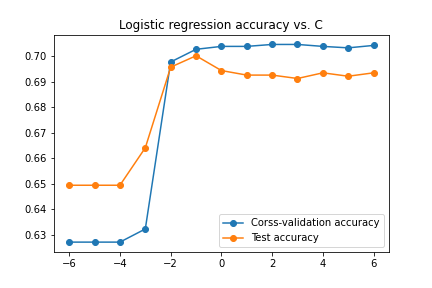
\includegraphics[width=6in,height=0.3\textheight]{figures/lr1} 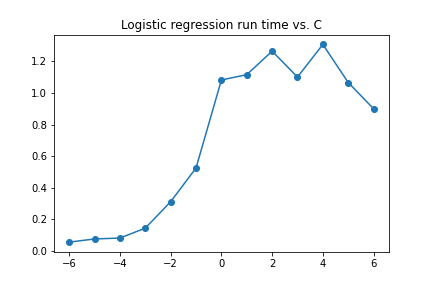
\includegraphics[width=6in,height=0.3\textheight]{figures/lr2} 

}

\caption{Plots of Logistic Regression}\label{fig:unnamed-chunk-11}
\end{figure}

\begin{figure}

{\centering 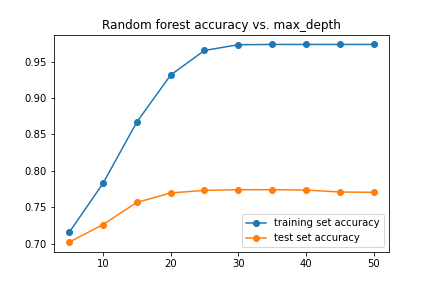
\includegraphics[width=6in,height=0.3\textheight]{figures/rf} 

}

\caption{Plots of Random Forest}\label{fig:unnamed-chunk-12}
\end{figure}

\begin{center}\includegraphics{report_files/figure-latex/unnamed-chunk-13-1} \end{center}





\newpage
\singlespacing 
\bibliography{master.bib}

\end{document}
